\chapter{實驗與執行結果}
%\label{c:intro}
本章節討論網頁與分析的結果與輸出數據
\section{網頁平台數據結果}
\subsubsection{顯示頁面}
在網頁的平台只有觀察使用者打字與紀錄時間並畫圖顯示。(圖4.11)為網頁偵測的頁面,有一空白處就是給使用者打字的地方,並且在進行打字同時計算字術語時間回傳,進而畫出時間字數的折線圖。
	\begin{figure}[H] 
	\centering 
	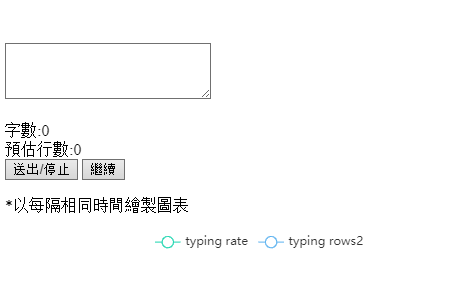
\includegraphics[width=0.7\textwidth]{4_1.png} 
	\caption{網頁顯示頁面} 
	\label{Fig.4.1} 
	\end{figure}
\subsubsection{網頁的圖形輸出}
因本研究是基於討論學生在做題目的分析,於是我找了一些文字試打並擷取回傳的圖形畫面結果:
\begin{enumerate}[1.]
	\item 簡短程式碼(圖4.2)
	\begin{figure}[H] 
		\centering 
		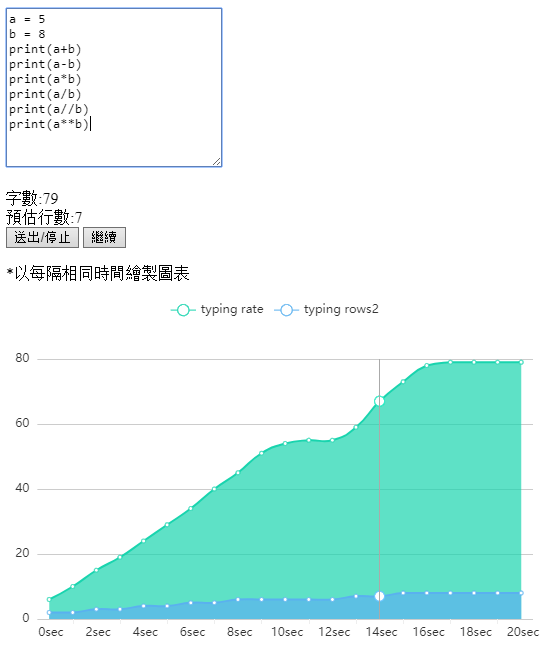
\includegraphics[width=0.7\textwidth]{4_2.png} 
		\caption{簡短程式碼輸出} 
		\label{Fig.4.2} 
	\end{figure}
	\item 簡短中文字(圖4.3)\\
	在打中文字時我所打錯的地方較多,所以使用backspace倒退鍵的情況也變多了,所以圖上呈現才會有更多的彎曲;上升一點下降一點就是使用者在改錯的地方。
	\begin{figure}[H] 
		\centering 
		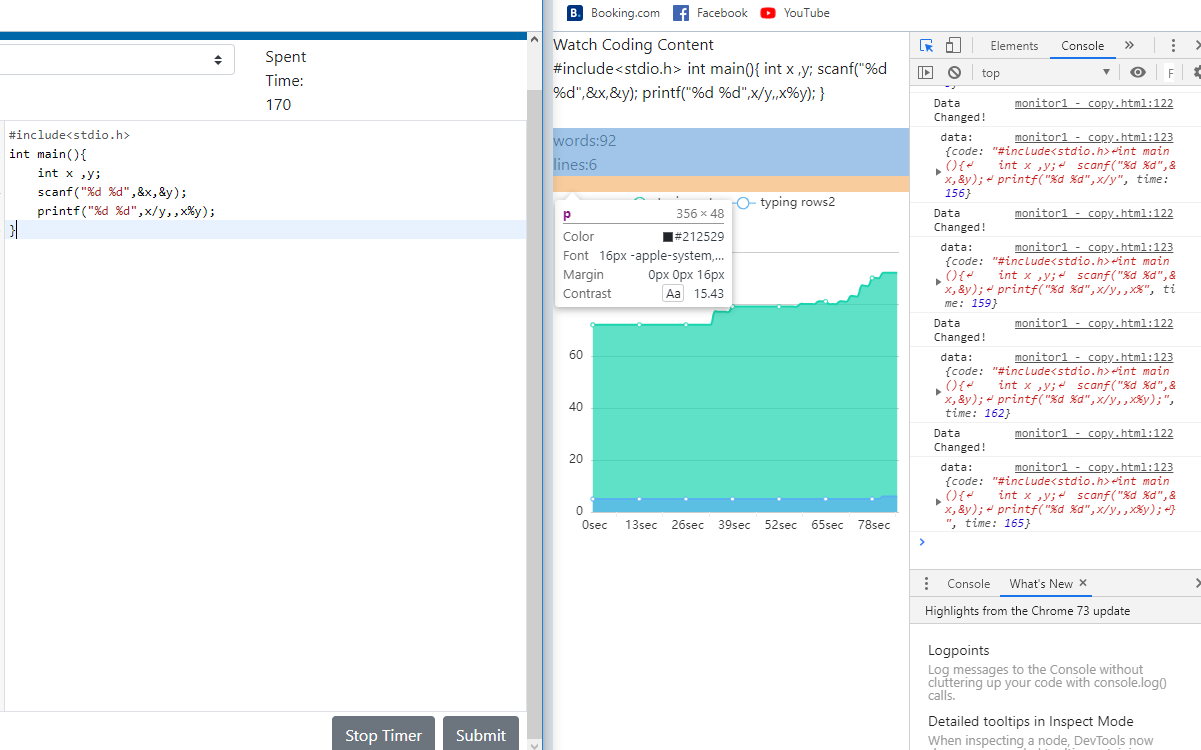
\includegraphics[width=0.7\textwidth]{4_3.png} 
		\caption{簡短中文字輸出} 
		\label{Fig.4.3} 
	\end{figure}
	\item 複製貼上(圖4.4)\\
	若是使用者貼上大量文字的話,圖形變化會成階梯狀因數據變化的幅度比自行打字大很多,因此如使用者使用了貼上鍵,此頁面是能夠偵測到的。
	\begin{figure}[H] 
		\centering 
		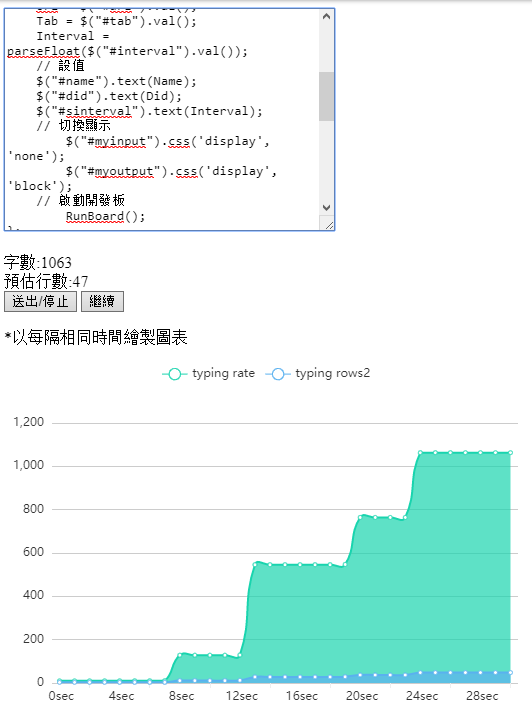
\includegraphics[width=0.7\textwidth]{4_4.png} 
		\caption{複製貼上輸出} 
		\label{Fig.4.4} 
	\end{figure}
\end{enumerate}
\section{python的討論分析}
因本研究所寫的python程式碼可以指定實驗數據的數量進進行製作與分析,在此便指定10組與30組結果。
\subsubsection{個別的圖形與數據}
每一組數據便會產生(圖4.5)的一組圖形,在此便不把全部圖形列出,以下只列每次產生的數據最基本的折線圖,共10組。(圖4.6)
	\begin{figure}[H] 
	\centering 
	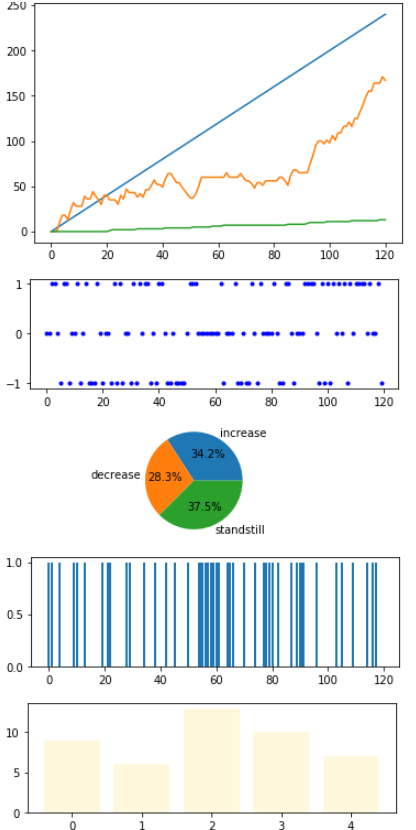
\includegraphics[width=0.7\textwidth]{4_5.png} 
	\caption{圖形組} 
	\label{Fig.4.5} 
	\end{figure}
	\begin{figure}[H] 
	\centering 
	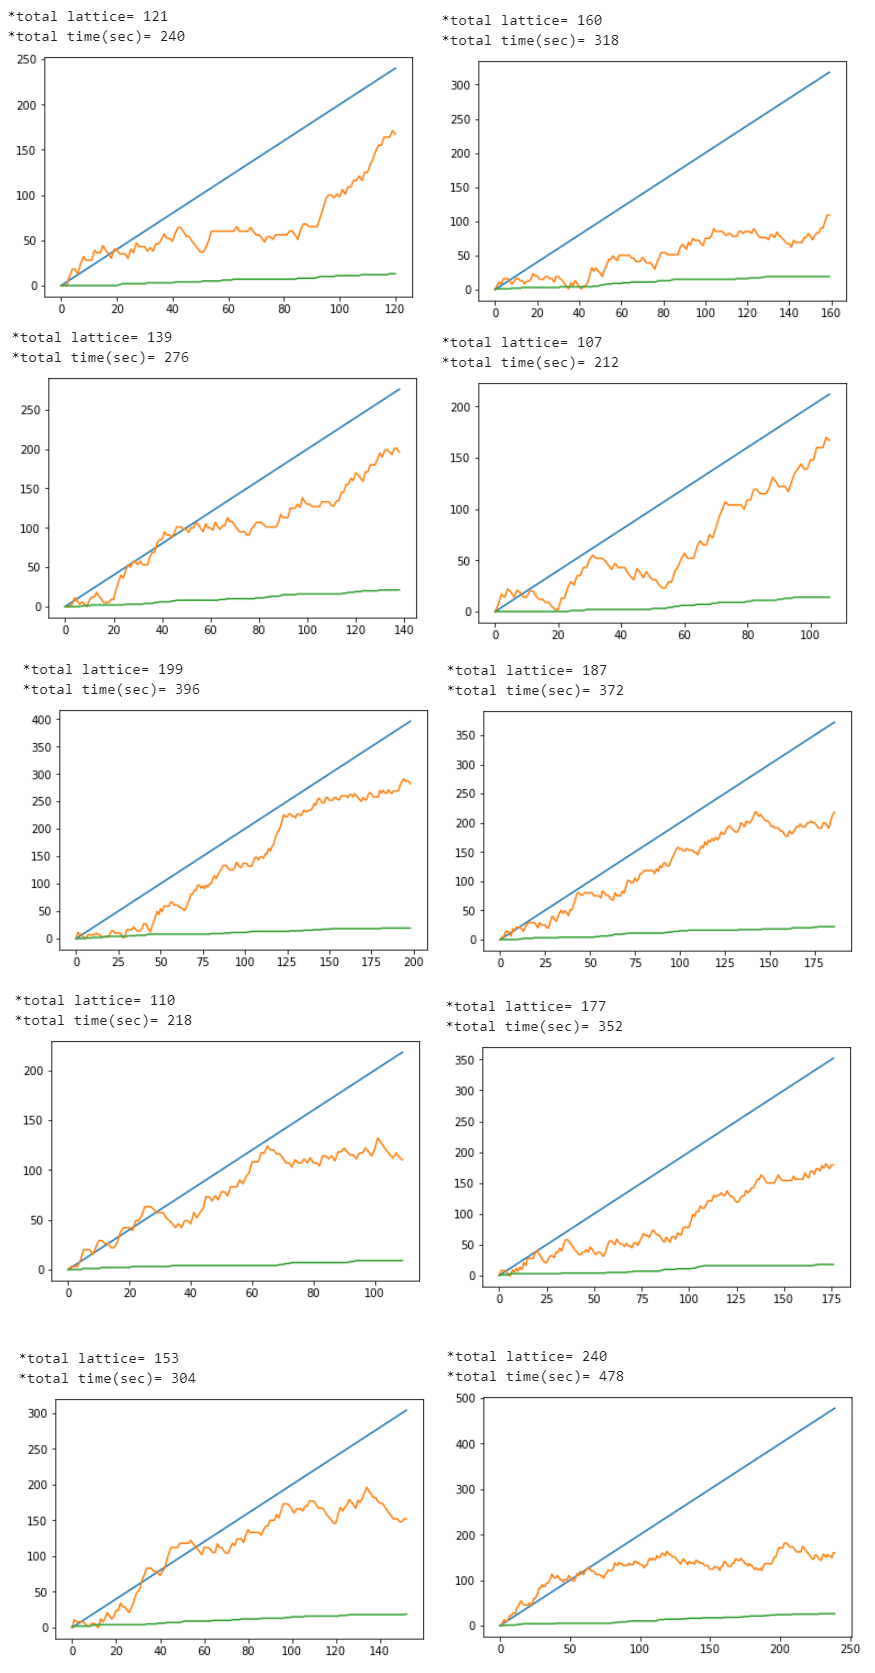
\includegraphics[width=0.7\textwidth]{4_6.png} 
	\caption{10組折線圖} 
	\label{Fig.4.6} 
	\end{figure}
\subsubsection{統整的表格數據}
把全部的數據統整起來製程表格,表格也是使用python在colab可以輸出顯示結果。\\
1. 10組結果(圖4.7)
	\begin{figure}[H] 
	\centering 
	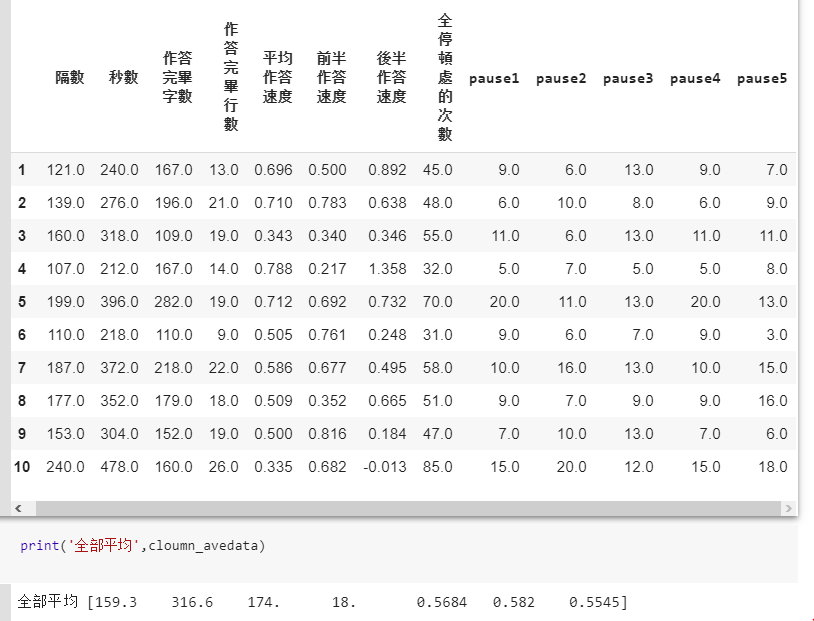
\includegraphics[width=0.7\textwidth]{4_7.png} 
	\caption{10組結果表格圖} 
	\label{Fig.4.7} 
	\end{figure}
\newpage
2. 30組結果,因資料較龐大所以使用表格顯示(表4.1))\\
\begin{table}[]
	\label{table1}
	\begin{tabular}{lllllllll}
		& 隔數  & 秒數  & 作答完畢字數 & 作答完畢行數 & 平均作答速度 & 前半作答速度 & 後半作答速度 & 全停頓處的次數 \\
		1  & 115 & 228 & 193    & 19     & 0.846  & 0.833  & 0.86   & 39      \\
		2  & 190 & 378 & 343    & 14     & 0.907  & 0.984  & 0.831  & 72      \\
		3  & 212 & 422 & 230    & 26     & 0.545  & 0.417  & 0.673  & 69      \\
		4  & 149 & 296 & 204    & 12     & 0.689  & 0.716  & 0.662  & 52      \\
		5  & 172 & 342 & 246    & 17     & 0.719  & 0.374  & 1.064  & 53      \\
		6  & 135 & 268 & 94     & 15     & 0.351  & 0.425  & 0.276  & 46      \\
		7  & 219 & 436 & 299    & 26     & 0.686  & 0.583  & 0.789  & 67      \\
		8  & 133 & 264 & 189    & 19     & 0.716  & 0.803  & 0.629  & 51      \\
		9  & 111 & 220 & 171    & 11     & 0.777  & 1.509  & 0.045  & 31      \\
		10 & 127 & 252 & 80     & 15     & 0.317  & 0.516  & 0.119  & 47      \\
		11 & 140 & 278 & 242    & 19     & 0.871  & 0.964  & 0.777  & 51      \\
		12 & 241 & 480 & 288    & 26     & 0.6    & 0.354  & 0.846  & 77      \\
		13 & 222 & 442 & 371    & 25     & 0.839  & 1.009  & 0.67   & 70      \\
		14 & 220 & 438 & 288    & 28     & 0.658  & 0.749  & 0.566  & 71      \\
		15 & 247 & 492 & 218    & 28     & 0.443  & 0.472  & 0.415  & 84      \\
		16 & 158 & 314 & 176    & 18     & 0.561  & 0.924  & 0.197  & 52      \\
		17 & 162 & 322 & 136    & 17     & 0.422  & 0.472  & 0.373  & 61      \\
		18 & 227 & 452 & 267    & 29     & 0.591  & 0.633  & 0.549  & 81      \\
		19 & 199 & 396 & 139    & 19     & 0.351  & 0.641  & 0.061  & 75      \\
		20 & 240 & 478 & 209    & 32     & 0.437  & 0.552  & 0.322  & 75      \\
		21 & 202 & 402 & 178    & 25     & 0.443  & 0.597  & 0.289  & 61      \\
		22 & 189 & 376 & 349    & 22     & 0.928  & 0.793  & 1.064  & 53      \\
		23 & 203 & 404 & 161    & 26     & 0.399  & 0.302  & 0.495  & 65      \\
		24 & 146 & 290 & 197    & 8      & 0.679  & 1.186  & 0.172  & 48      \\
		25 & 195 & 388 & 185    & 17     & 0.477  & 0.629  & 0.325  & 70      \\
		26 & 93  & 184 & 61     & 10     & 0.332  & 0.946  & -0.283 & 25      \\
		27 & 98  & 194 & 60     & 2      & 0.309  & 0.33   & 0.289  & 28      \\
		28 & 93  & 184 & 132    & 8      & 0.717  & 0.772  & 0.663  & 33      \\
		29 & 204 & 406 & 225    & 18     & 0.554  & 0.951  & 0.158  & 65      \\
		30 & 120 & 238 & 91     & 16     & 0.382  & 0      & 0.765  & 52     
	\end{tabular}
\caption{30組數據}
\end{table}
\newpage
\section{結果討論}
\subsection{html網頁偵測部份}
\begin{itemize}
	\item 本研究藉由網頁前端及時偵測使用者的打字情況,並且計算其字數與花費時間。不同於其餘答題系統需要繳交後才知曉使用者的答題狀況,此方法因為其實時偵測的特性,使用者的答題習慣也可以藉由字數與時間看出端倪。
	\item 在網頁上只擷取了字數、行數與時間,如可以增加更多的鍵盤偵測將會使系統更加完善,此處為能多加以改良完善的地方。
\end{itemize}
\subsection{python分析部分討論}
\begin{itemize}
	\item 進行分析的部分最大的難處就是缺少實際數據,因此在本文中使用程式去模擬實際的數據。但是因在此使用大量的radom函數與諸多限制,如為了使程式撰寫方便設的上下界線使數據密集化等。模擬的數據理所當然地不及實際數據來的真實與客觀。
	\item 再討論數據停頓的密集程度的地方(圖3.16),我所選用的方法是把整體數據分成五個等分並寫計算每一等分的停頓次數;而此部分也是不夠嚴謹的,因可能密集的地方會被分組計算而分割,所以分區計算的方法並不能表示絕對的疏密程度。
\end{itemize}